\begin{figure}[t]
  \centering
  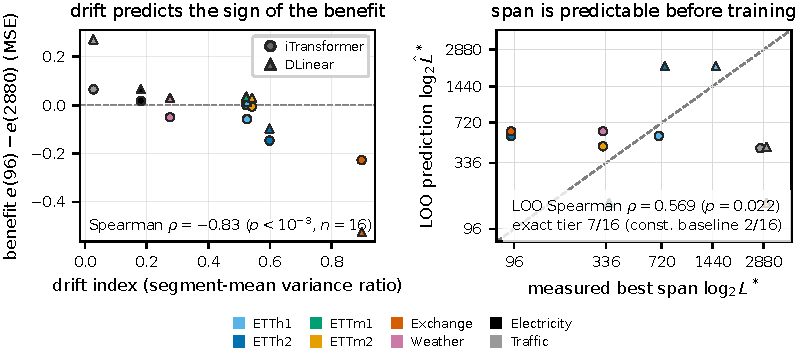
\includegraphics[width=0.52\linewidth]{figs/fig2_predictability.pdf}
  \caption{The effective span is predictable from training-free context statistics computed on the train split only. Left: drift index versus measured long-context benefit across the eight main-suite benchmarks and two model families (Spearman $\rho = -0.83$ over the sixteen samples; cluster-level reading over the eight datasets $\rho = -0.88$, $p = 0.004$). Right: leave-one-dataset-out predicted versus measured log-span (main-suite panel; the enlarged fourteen-dataset suite of Section \ref{sec:predictfull} gives $\rho = 0.63$; dashed line is identity).}
  \label{fig:predict}
\end{figure}
